\documentclass[DM,toc,lsstdraft]{lsstdoc}

\title[Heterogeneous Focal Plane]{Impact of a Heterogeneous Focal Plane on LSST Image Differencing}

\author{C. T. Slater, R. L. Jones, E. Bellm, and M. Juri\'c}

\setDocRef{LDM-523}
\date{\today}

\setDocAbstract{%
The LSST heterogeneous focal plane is a potential source of false detections in image
differencing due to difference between vendors in the sensor quantum
efficiencies as a function of wavelength. We can evaluate the magnitude of this
effect in a worst-case scenario (with no attempt at correction) by estimating
the flux difference that would be measured between sensors, for a variety of
stellar SEDs, and combining this with the expected density of sources at a given
color and the probability that they will exceed the 5$\sigma$ detection
threshold as a result of the measurement difference. Overall the sensor
differences are small enough that only negligible numbers of false detections
will result, but we note that the specifications for the filter transmission
curve currently permit a level of spatial variations that could lead to a
significant number of false detections.
}

\setDocChangeRecord{%
\addtohist{1}{2017-05-12}{Initial version.}{Colin Slater}
}

\begin{document}
\maketitle

\section{Executive Summary}

If the LSST focal plane is comprised of sensors from multiple vendors, it is
likely that they will differ in quantum efficiency as a function of wavelength \citedsp{Report-241}.
Based on preliminary throughput curves derived in early 2017 from engineering
models, the g-band exhibits the greatest difference between the two vendors,
particularly in the shape of the throughput curve. Thus the measured flux of an
object observed with one vendor's sensor will differ from that measured on the
other type of sensor, and the magnitude (and direction) of this effect will
depend on the spectral energy distribution of the object.

This problem is analogous to the issue of differential chromatic refraction (DCR),
where a similar sensitivity to the object's SED appears when an object is
observed at varying airmass. DCR is very challenging since it induces an
astrometric shift in addition to a photometric difference. DCR has been long
identified as a significant challenge for Data Management, and efforts at
developing algorithms to correct for this effect are underway. It is very likely
that an extension of the same algorithms designed for correcting DCR will also
be able to correct for the different sensor response curves, since they both
require estimating the coarse intra-band SED, then generating an appropriately
corrected template for image differencing. This would be the ideal solution for
handling the mixed-vendor focal plane.

We have also sought to characterize the degradation of image differencing
performance if a heterogeneous focal plane was used without such an algorithm in place.
A significant concern is that images of an object from one sensor type may be
differenced against a template built from the other sensor type, leading to an
artificial difference in flux that would be reported as a \DIASource even if the
object is unvarying. If this occurs for a large number of objects it could
degrade the purity of the Level 1 alert stream, add excessive computational
cost, and potentially hamper the linking of moving object detections into
\SSObjects.

We have evaluated the magnitude of the flux difference in g-band for various
stellar SEDs. The shift can be ``calibrated out'' for stars of a mean color,
since they will statistically set the zeropoint difference between the two
exposures. But stars significantly bluer or redder than this mean color will
still exhibit flux shifts, and these are generally of order 5-10\,mmag at most.
To determine how many stars fall into these red and blue wings, we use a
measured stellar color distribution from SDSS. For most faint stars
this shift will be lost in Poisson noise of the measurement, but bright stars
will be measured well enough they will be more likely to cross the 5$\sigma$
threshold to be reported as a \DIASources. We therefore modeled a distribution
of observed stellar magnitudes plus a model of the photometric uncertainties for
stars with a given brightness and spurious flux difference (from the heterogeneous focal
plane) to estimate the total number of false positives per square degree.

The results from this exercise show that the worst-case false detection rates
from the heterogeneous focal plane are roughly 1-10 per square degree, depending on
whether the field is at low or high Galactic latitude. This is below the
irreducible level of detections from pure background noise of roughly 60 per square degree.
We therefore do not believe that the heterogeneous focal plane will present a problem
for image differencing.

However, the false positive rate rises very steeply with any such coherent
difference in flux between images. The filters are another potential source of
such differences, as localized variation in coatings could lead to a similar
dependence on object SED as described above. Based on the filter transmission
curve specifications, the magnitude of this effect is potentially much larger
than the differences between sensors. The wavelengths of the filter bandpass
edges are permitted to vary by up to 1.5\%, which in g-band would cause
photometric differences as large as 15-20\,mmag for a significant number of
objects. This could potentially create false positives at rates of 100s per
square degree. Expected rates of astrophysical transients are of a similar order
of magnitude, which makes this a significant concern.

\section{Analysis}

\subsection{Predicting Flux Differences}

The software available in the sims packages and LSST \code{throughputs} package
can compute observed magnitudes for given SEDs by integrating the flux under a
specified set of component transmission curves. We examined two scenarios, one
with a sensor difference, and one with a filter difference. For the sensor
difference scenario, the transmission curves were the baseline values from
\code{throughputs}, except the sensor QE curves have been replaced with the
as-measured values from the two vendors. The difference in flux between the two
cases (vendor 1 and vendor 2) is shown in Figure~\ref{fig:delta_g_vs_color}, as
computed for a few stellar SEDs. The second scenario compares the fluxes from
the baseline set of throughputs vs. the baseline with a substituted g-band
filter transmission curve, which had been shifted in wavelength by 1\%. This is
less than the specification on the filter transmission edges (OSS-REQ-0238,
\texttt{filtUniformity\_grizy}\ossreq{0238}), which allow up to 1.5\% variation
in the bandpass edges over the filter aperture.

\begin{figure}
\centering{%
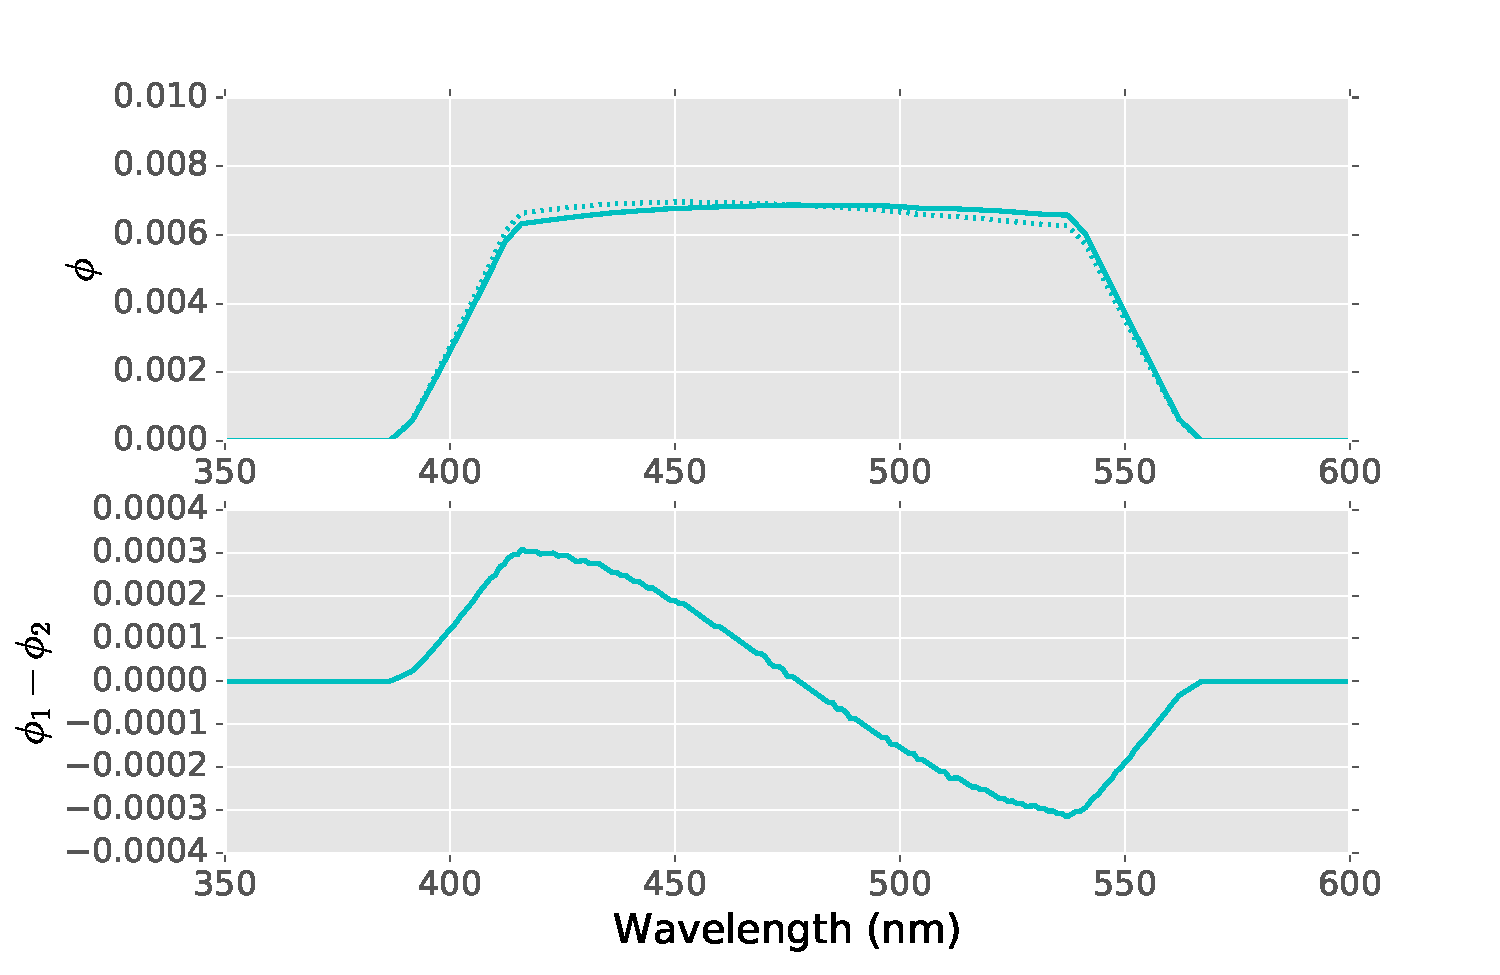
\includegraphics[width=0.8\textwidth]{figures/QE_response_curves.pdf}
}
\caption{Normalized g-band response curves for sensors from the two vendors
(top), and the difference of these two curves (bottom).
\label{fig:QE_response_curves}
}
\end{figure}

\begin{figure}
\centering{%
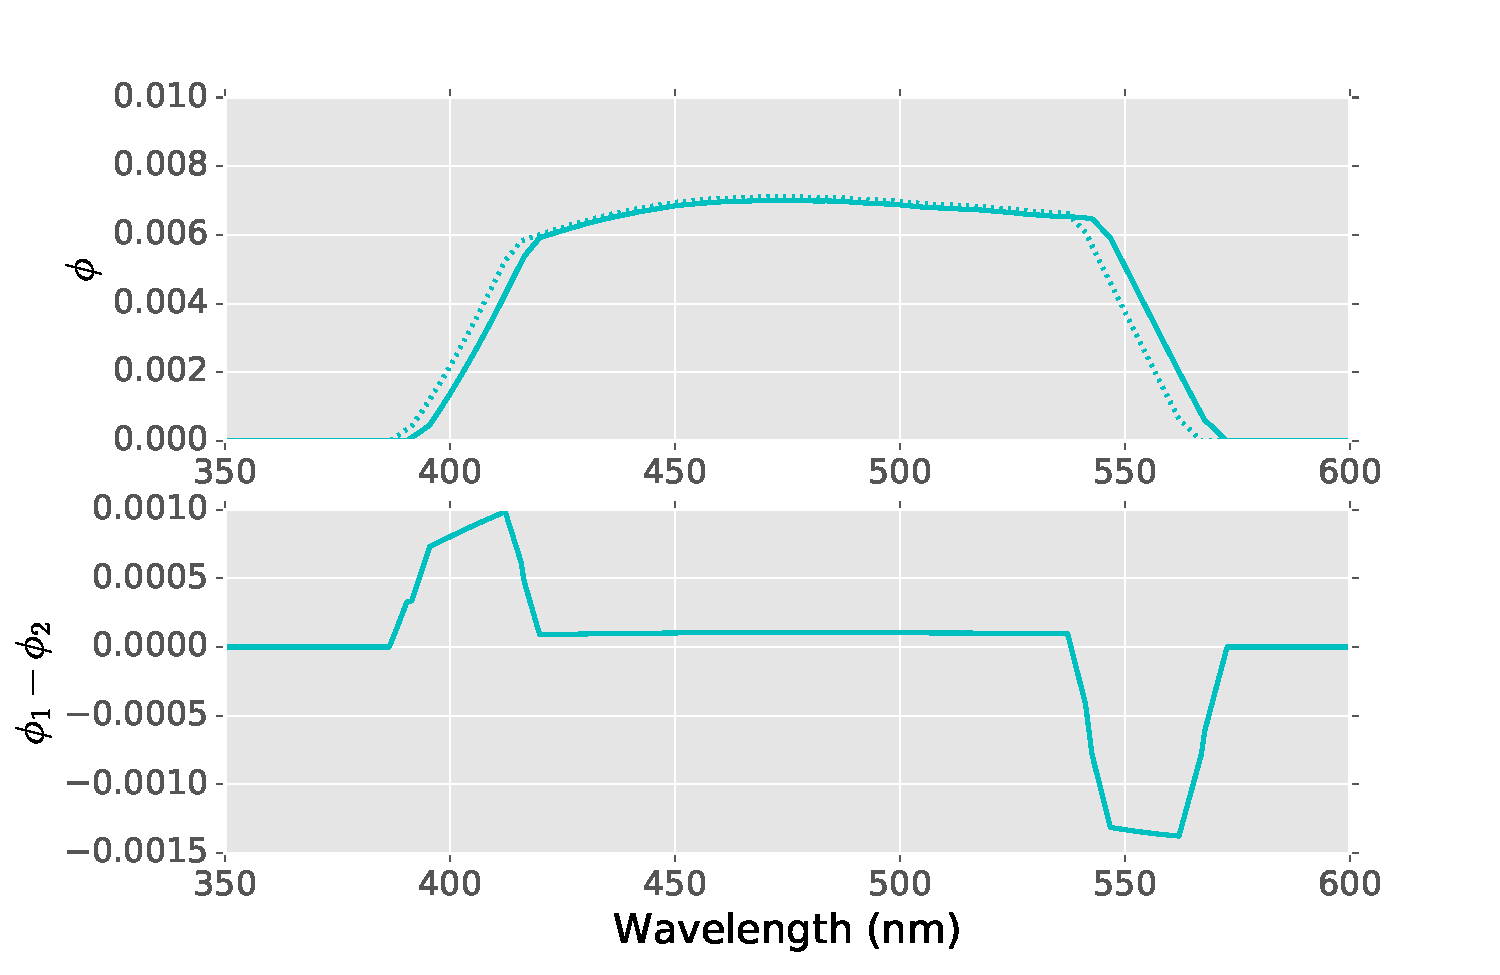
\includegraphics[width=0.8\textwidth]{figures/filter_response_curves.pdf}
}
\caption{Same as Figure~\ref{fig:QE_response_curves}, but for the baseline
g-band filter and the same filter shifted by 1.0\% in wavelength.
\label{fig:filter_response_curves}
}
\end{figure}

\begin{figure}
\centering{%
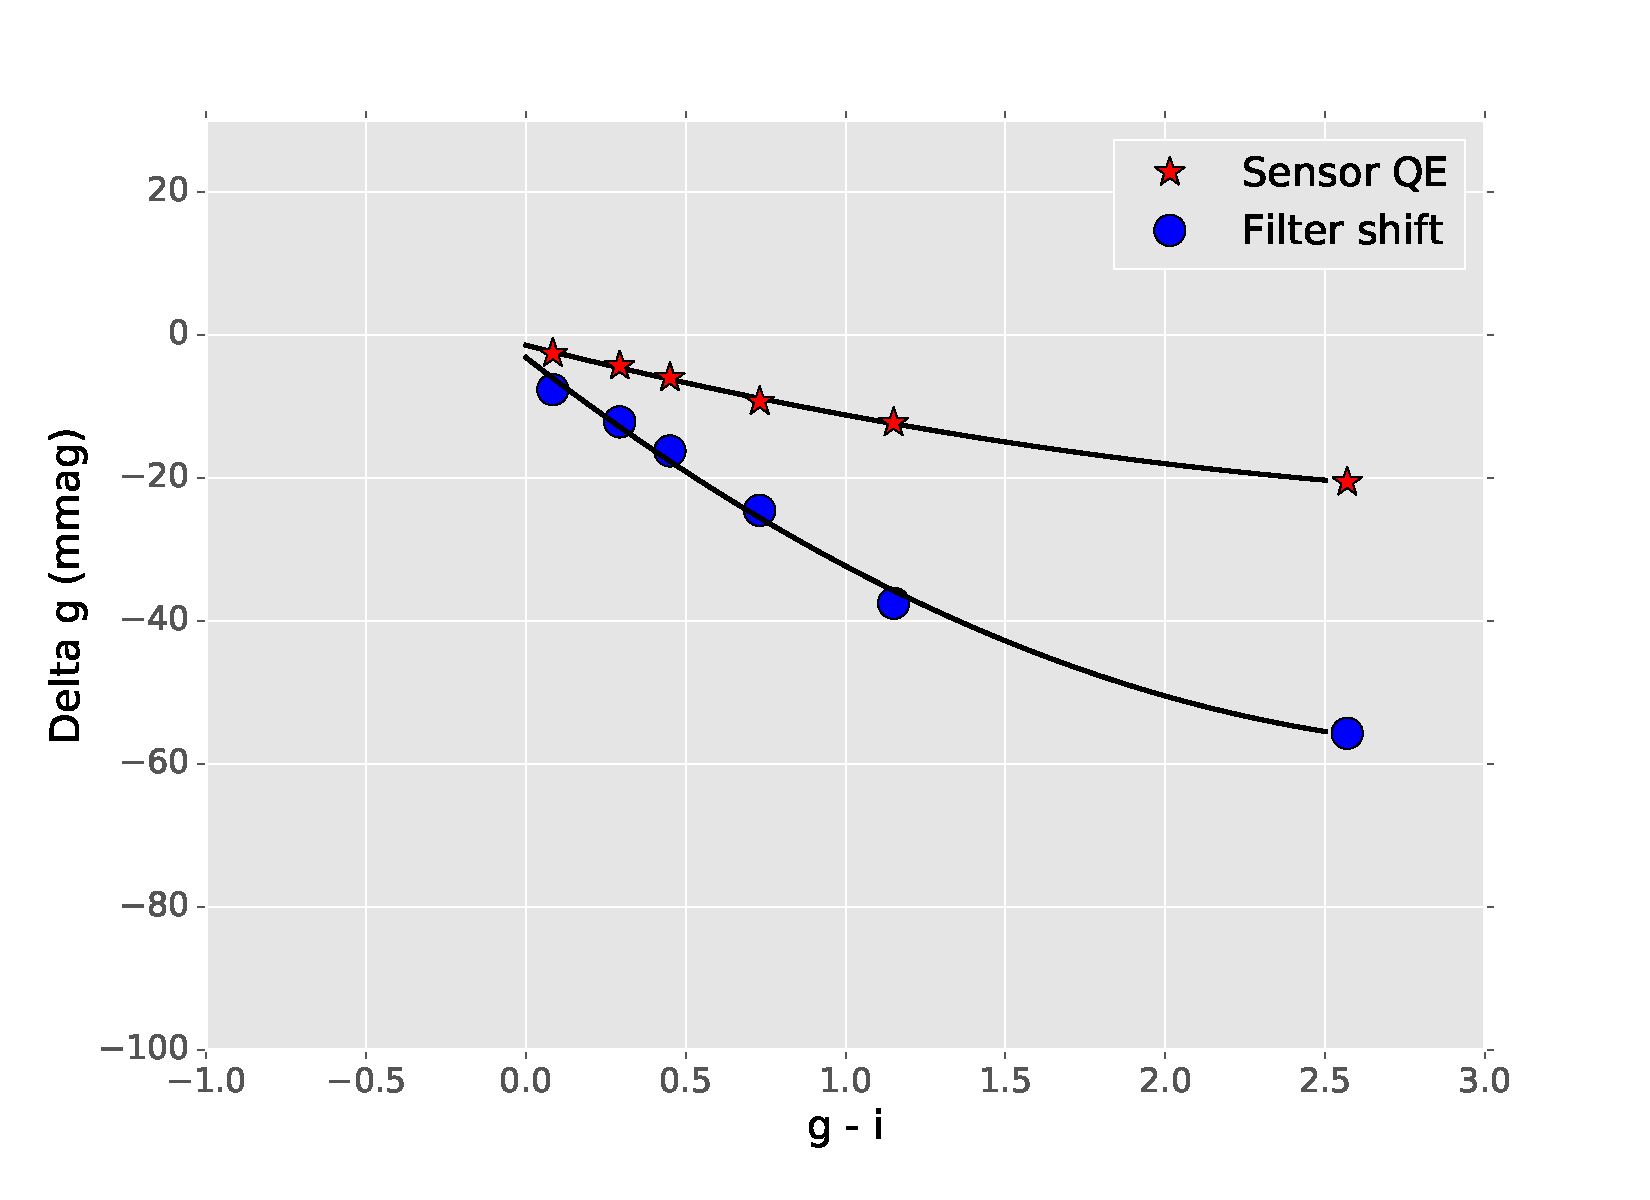
\includegraphics[width=0.9\textwidth]{figures/delta_g_vs_color.pdf}
}
\caption{Difference in g-band flux between measurements made on sensors from
different vendors (``Sensor QE'', red stars), and between two different
realizations of the g-band filter (``Filter shift''), where one filter
realization was the baseline specification and the other had both red and blue
cutoffs shifted by 1\% in wavelength (less than the 1.5\% specification). For
comparison we also show the color difference between images taken at airmass 1.0
and airmass 1.5, since this level of variation is unavoidable. Measured QE
curves from prototype sensors (as of early 2017) were used in the sensor
comparison.
\label{fig:delta_g_vs_color}}
\end{figure}

The full-range of flux differences in Figure~\ref{fig:delta_g_vs_color} spans
$\sim$20\,mmag for the sensor case and $\sim$50\,mmag for the filter case. This
full span is not representative of the distribution of flux differences that
will be seen in an average image, since stars of some average color will have
this difference calibrated out when the images are photometrically scaled
together. To estimate the distribution of flux differences, we took a $g-i$
color histogram from SDSS Stripe 82 and used the fits shown in
Figure~\ref{fig:delta_g_vs_color} to transform this histogram into a g-band flux
difference. Figure~\ref{fig:delta_g_histogram} shows these histograms, where zero
shift is set to be at the mean $g-i$ color of stars in the histogram.

\begin{figure}
\centering{%
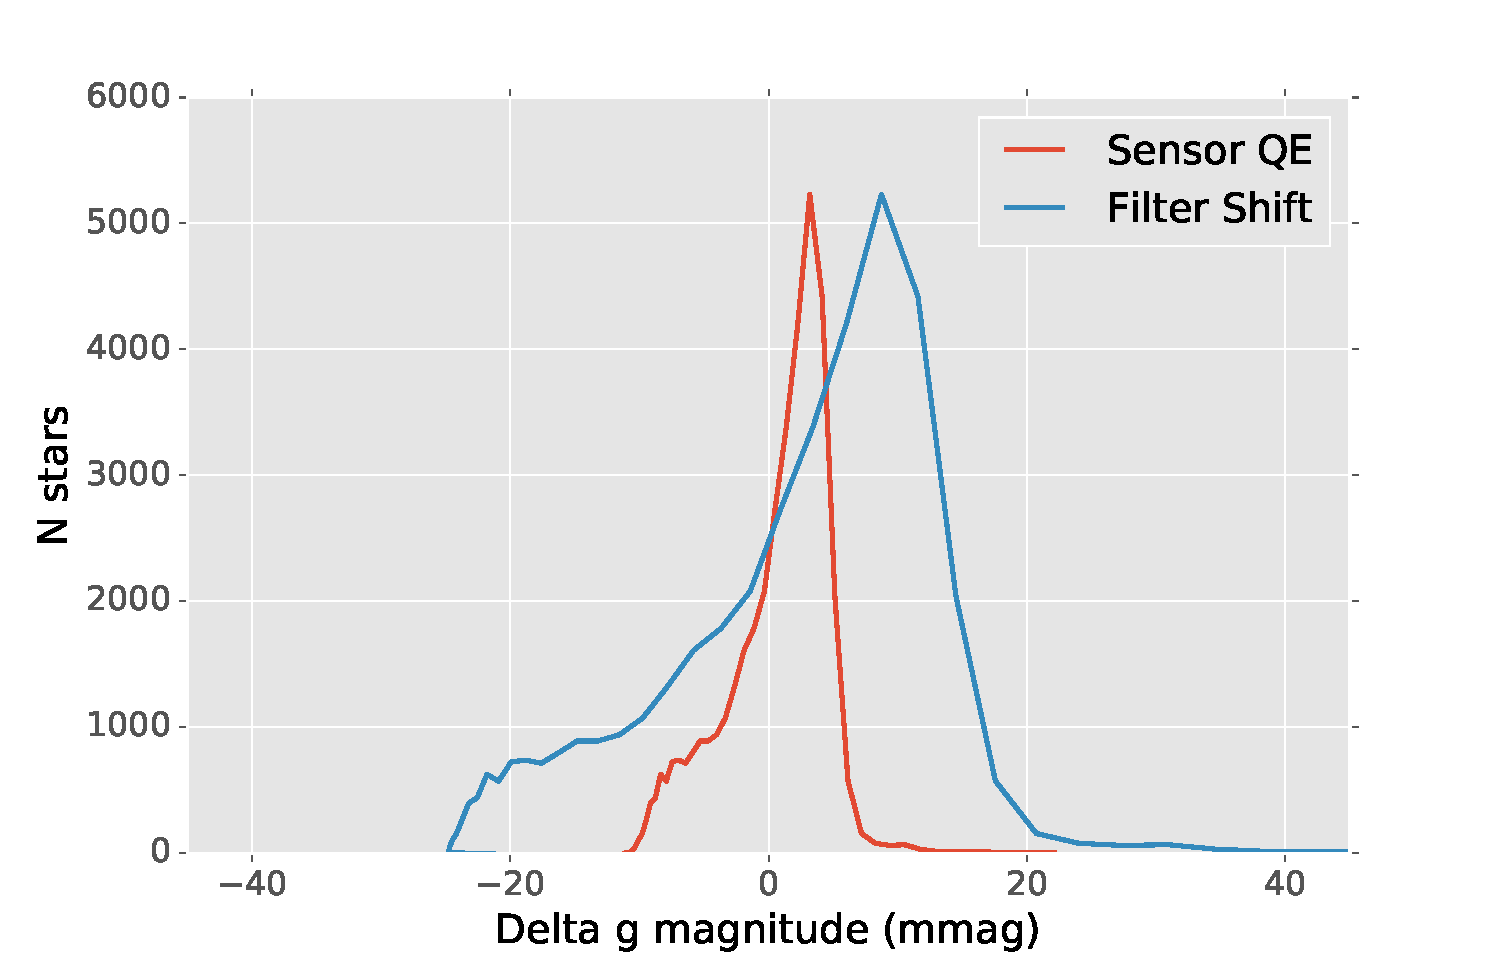
\includegraphics[width=0.9\textwidth]{figures/delta_g_histogram.pdf}
}
\caption{Distribution of g-band magnitude shifts that would be when stars with a
realistic $g-i$ color distribution were observed in the sensor and filter
scenarios described in Figure~\ref{fig:delta_g_vs_color}. The mean g-band
difference is corrected for when the two (hypothetical) images are matched in flux,
but very red or very blue stars will exhibit flux differences of up to $\sim$20\,mmag.
\label{fig:delta_g_histogram}}
\end{figure}

A cumulative version of this information is shown in
Figure~\ref{fig:delta_g_cumulative}. This shows the fraction of observed
stars that will have an absolute flux difference (discarding sign) greater than
a given level. The median difference is thus approximately 4\,mmag for the
different sensors, and 9\,mmag for the filter shift, but there are significant
tails particularly for the filter case.

\begin{figure}
\centering{%
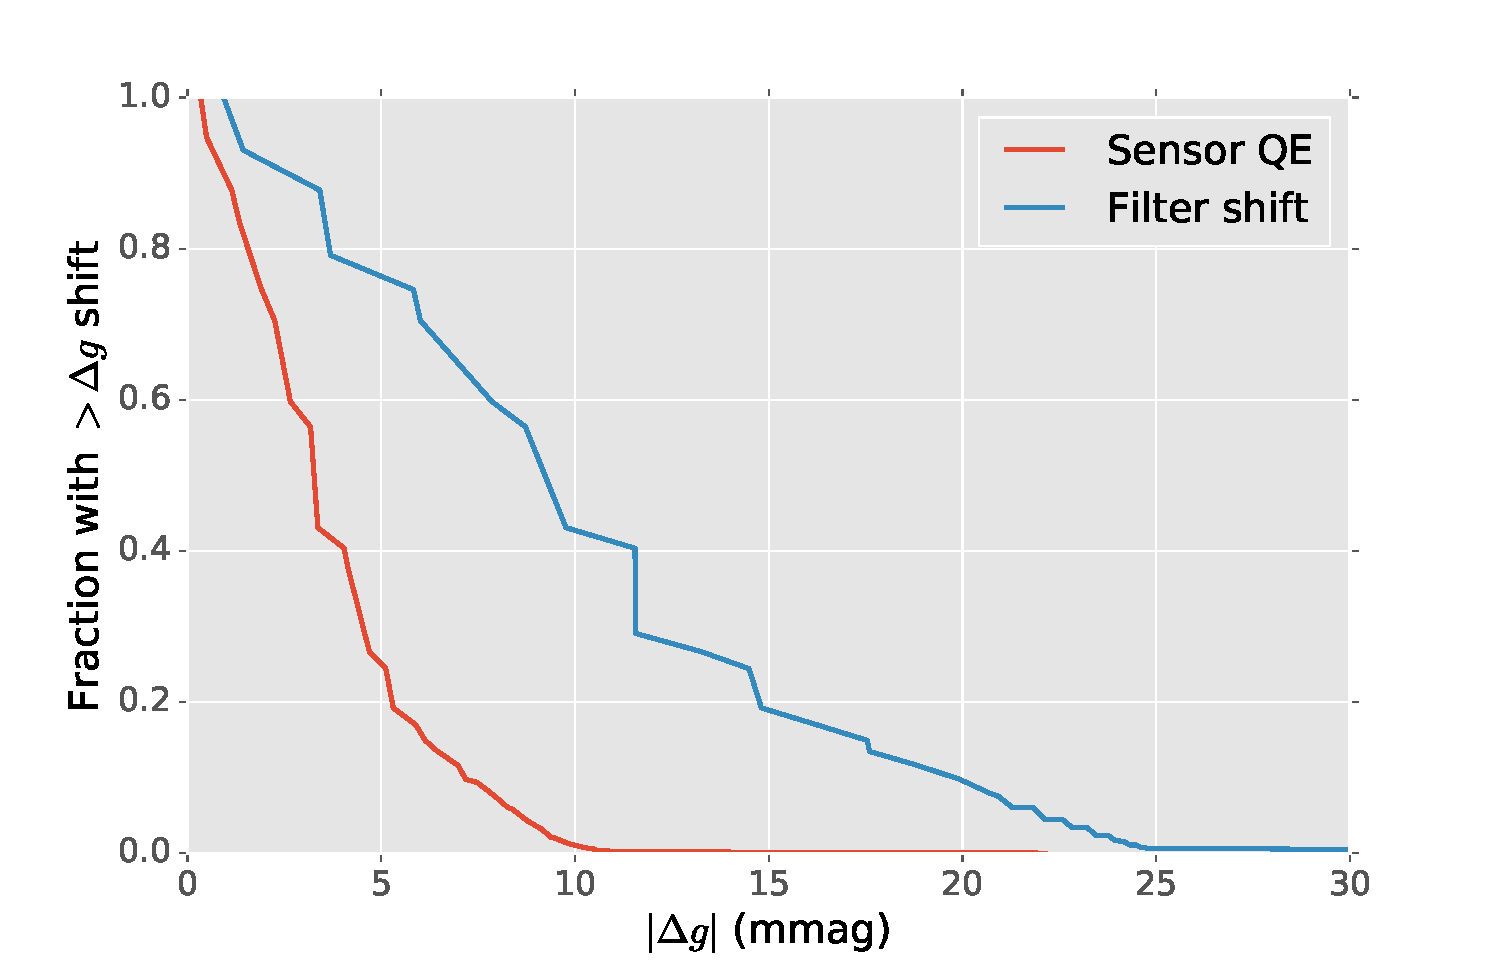
\includegraphics[width=0.9\textwidth]{figures/delta_g_cumulative.pdf}
}
\caption{Cumulative distribution of Figure~\ref{fig:delta_g_histogram}. Roughly
10-15\% of (unvarying) stars will exhibit $>$7\,mmag g-band differences when
images from the two sensor types are differenced, while 20\% of stars will show
differences of 15\,mmag or greater if imaged by different filter bandpasses.
\label{fig:delta_g_cumulative}}
\end{figure}


\subsection{False Positive Rates from Coherent Flux Differences}

The preceding section showed that some fraction of stars will exhibit spurious
flux differences if the images being compared were taken with two different
system throughputs. These differences are not large enough to consistently
appear as 5$\sigma$ detections in image differencing, but they will make stars
more likely to cross this 5$\sigma$ threshold due to Poisson noise. This is
because the threshold for detection is set by the noise level of the image
assuming that there is no mean flux difference. For a given threshold $\nu$
(e.g. 5), noise level $\sigma$, and flux difference $\delta$, the fraction of
detections that will exceed the threshold is given by
%
\begin{equation}
  f( > \nu, \delta) = 1 + \frac{1}{2}\textrm{erf}\left( \frac{-\nu - \delta/\sigma}{\sqrt{2}}\right) \
  - \frac{1}{2}\textrm{erf}\left( \frac{\nu - \delta/\sigma}{\sqrt{2}}\right).
\end{equation}
%
This function is plotted in Figure~\ref{fig:false_positive_prob}, where the flux
uncertainties have been computed for stars observed by a single LSST pointing
(including source noise for bright stars). When there is no coherent flux
difference, the detection probability is constant, but bright stars are
well-measured and are significantly more likely to be detected as \DIASources
when flux differences are present.

\begin{figure}
\centering{%
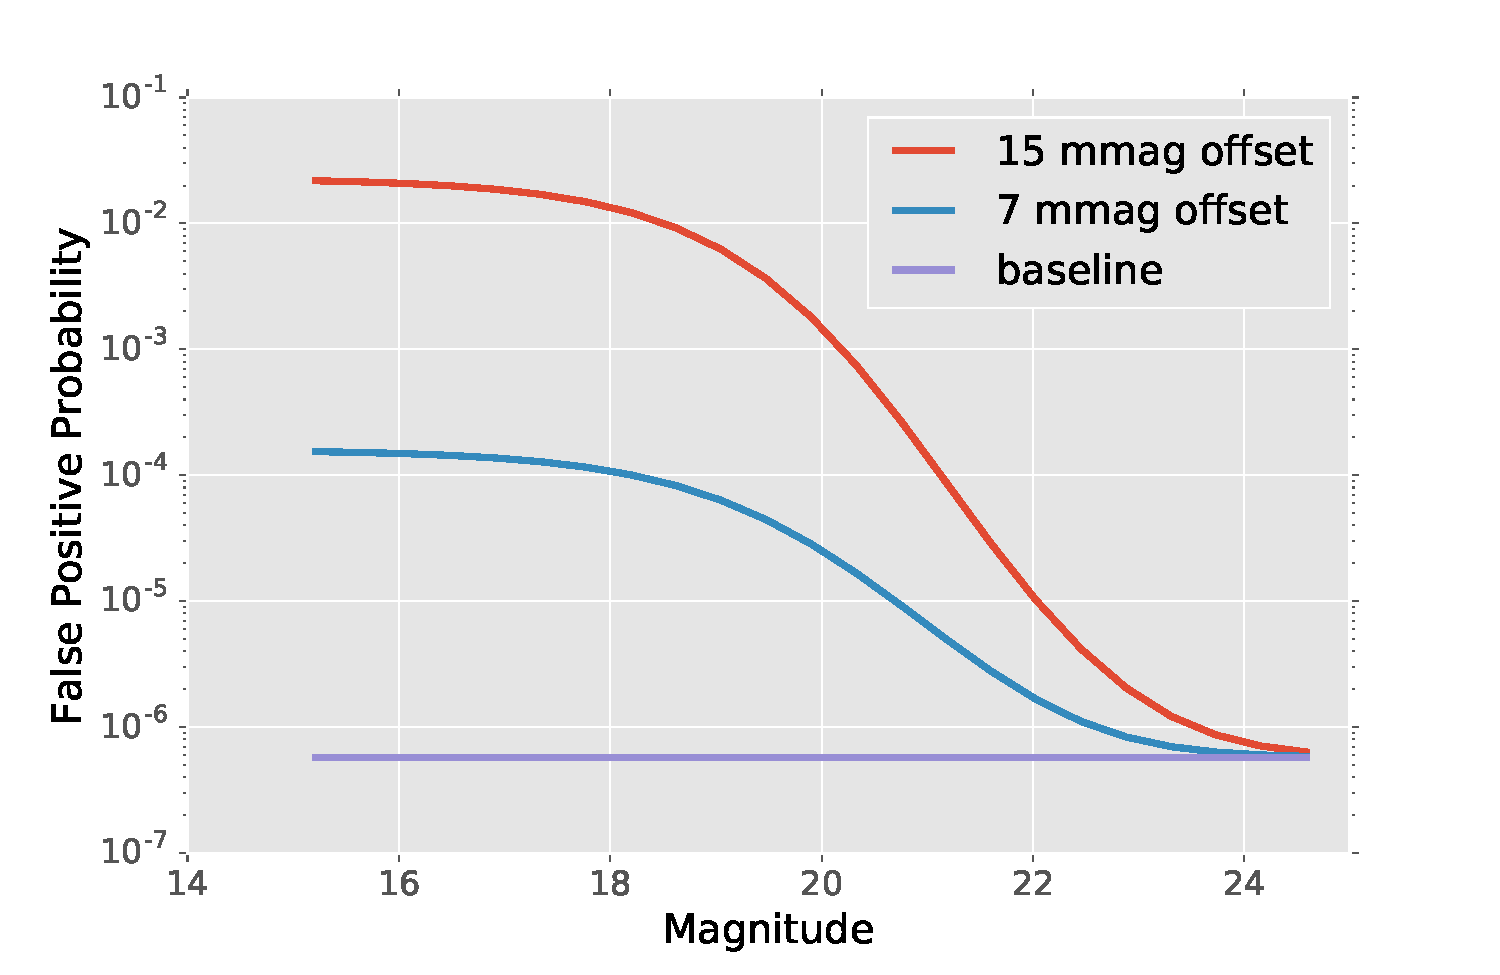
\includegraphics[width=0.9\textwidth]{figures/false_positive_prob.pdf}
}
\caption{Probability that a star at a given magnitude (unvarying) will be
measured as exceeding the 5$\sigma$ threshold for \DIASources, if there is a
coherent flux difference between the two images that are differenced. These
false positives are rejected at better than 1 in $10^6$ when the two images have
the same bandpass and sensor QE curves, but when there are variations in the
transmission curve, bright stars will be significantly more likely to exceed the
5$\sigma$ threshold.
\label{fig:false_positive_prob}}
\end{figure}

Figure~\ref{fig:false_positive_differential} multiplies this probability by the
number of stars (solid lines) and galaxies (dashed lines) expected per magnitude
in an LSST pointing. Stars brighter than 20th magnitude are the primary
contributors, and fainter than this level individual measurement noise makes the
flux differences unimportant.

\begin{figure}
\centering{%
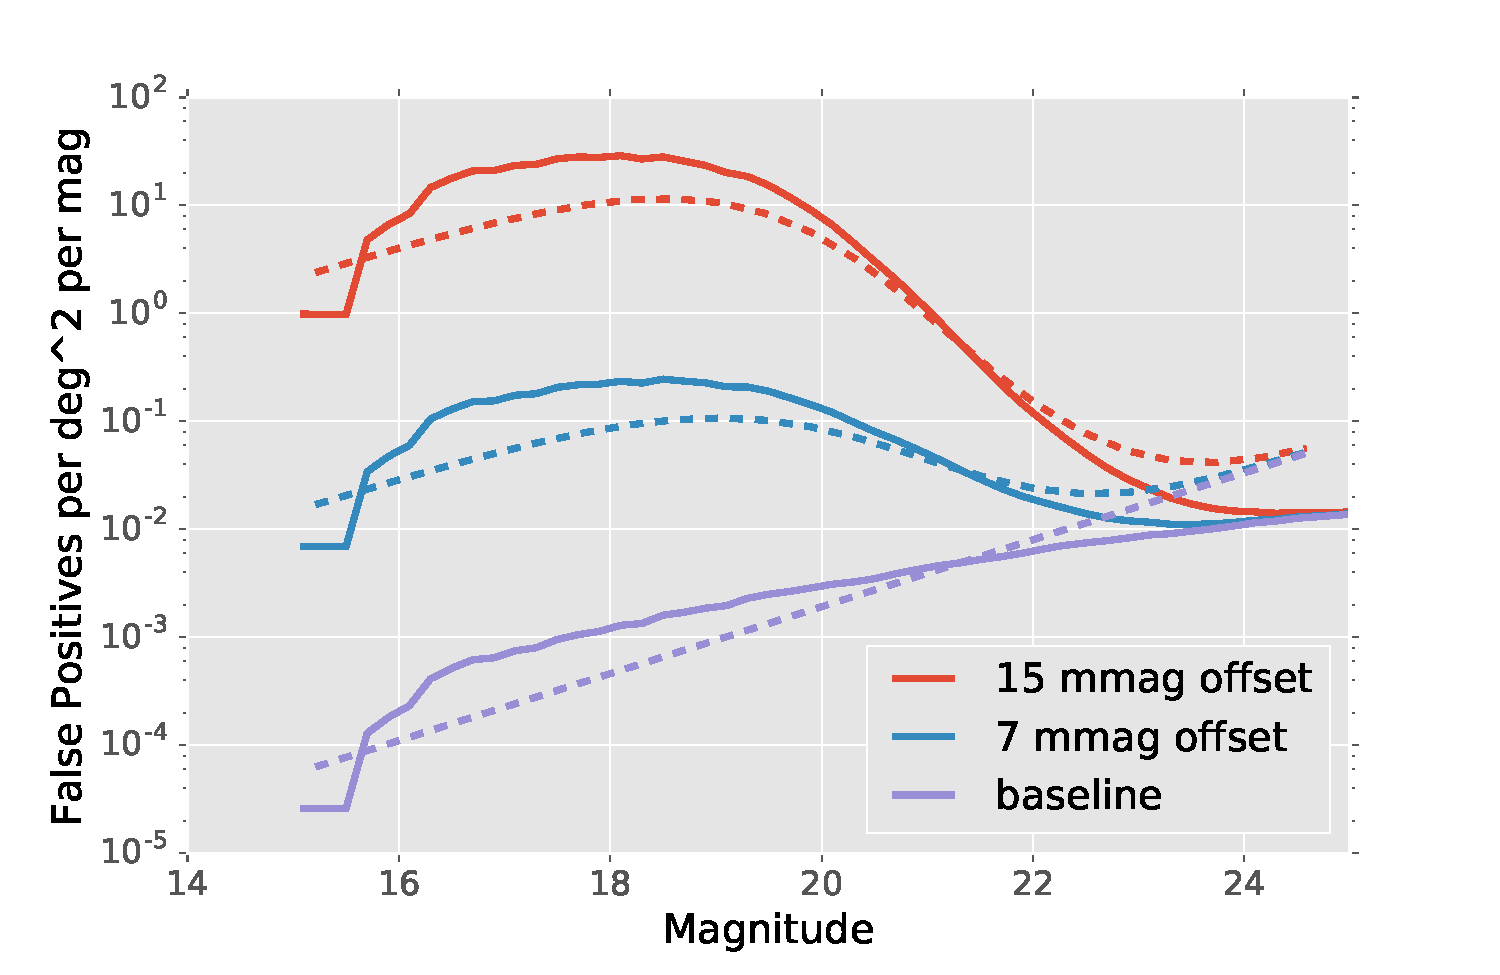
\includegraphics[width=0.9\textwidth]{figures/false_positive_differential.pdf}
}
\caption{This figure combines the false positive probabilities from
Figure~\ref{fig:false_positive_prob} with the number density of objects at a
given magnitude to show the total number of objects per square degree, per magnitude.
Solid lines show star counts (computed at $l=180^\circ$, $b=-45^\circ$), while
dashed lines show galaxies.
\label{fig:false_positive_differential}}
\end{figure}

\begin{figure}
\centering{%
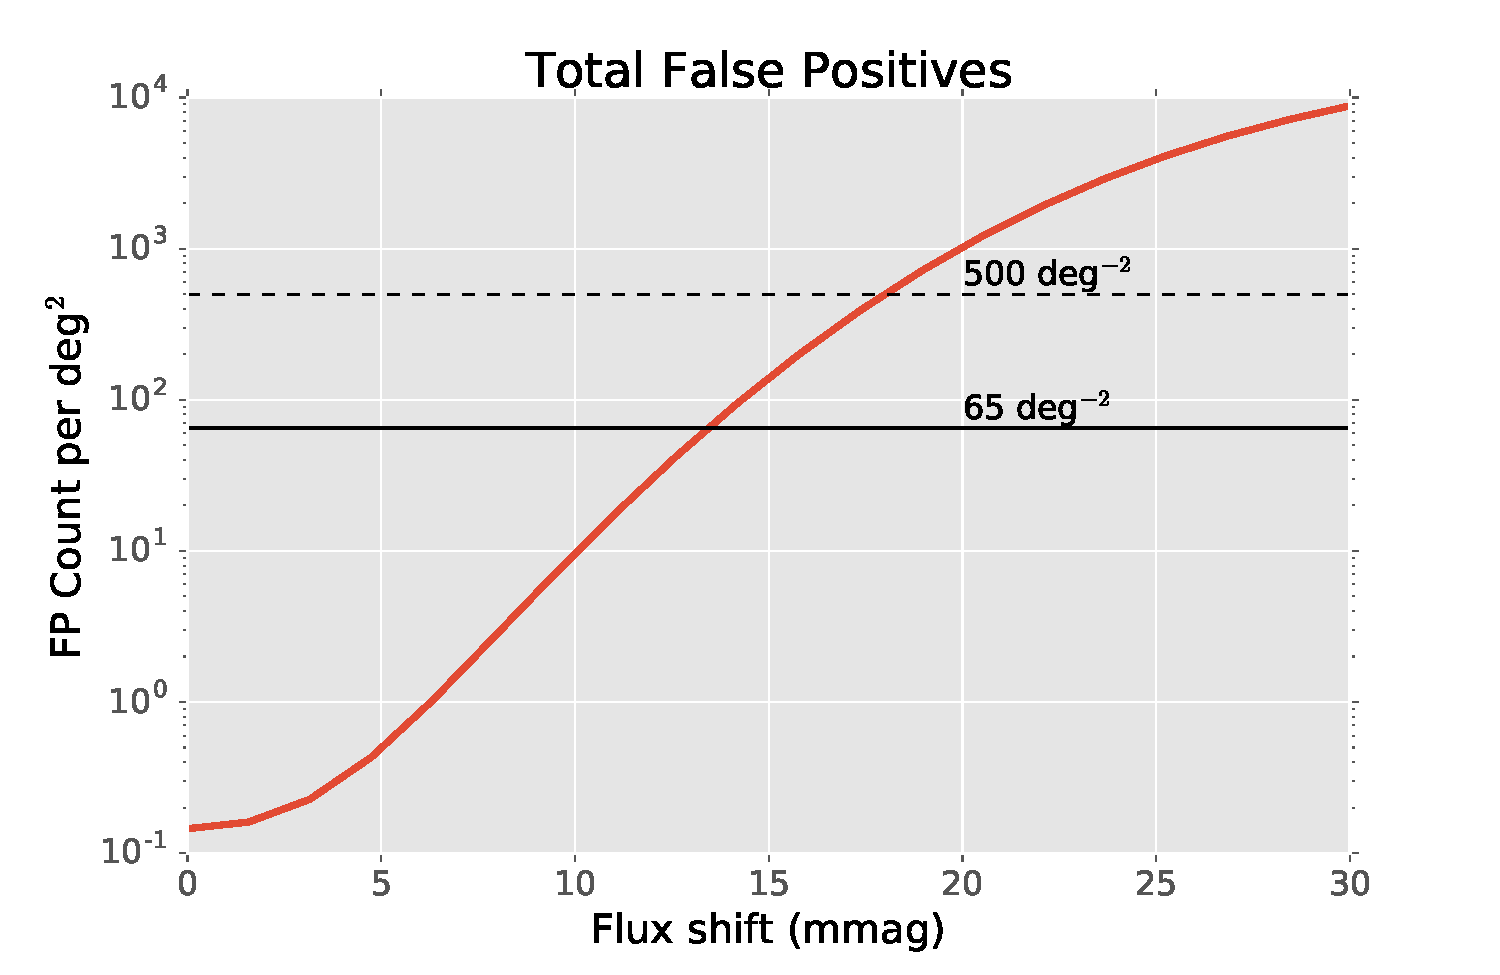
\includegraphics[width=0.9\textwidth]{figures/fp_vs_flux_shift.pdf}
}
\caption{Cumulative counts of false positives as a function of coherent flux
difference between observations. While shifts of up to 12\,mmag would not produce
more false positives than the irreducible background level of $\sim$65 per
square degree, greater shifts will would rapidly produce significant numbers of
false detections.
\label{fig:fp_vs_flux_shift}}
\end{figure}

The cumulative number of false positives (integrating each curve in
Figure~\ref{fig:false_positive_differential}) is shown in
Figure~\ref{fig:fp_vs_flux_shift}. For flux differences less than $\sim$14\,mmag,
the density of false positives is generally less than the density of false
detections from background noise (blank sky). However, the false detection rate
rises rapidly with increasing flux differences and can quickly grow into
hundreds per square degree, at which point it would become a dominant
contributor to the overall false positive rate.

\subsection{Conclusions}

These false positive densities in Figure~\ref{fig:fp_vs_flux_shift} can be combined
with the previous section, where we estimated that (e.g.) 10\% of stars
will have a 20\,mmag flux difference under the varying filter scenario. The
overall number is thus roughly 10\% of 1,000 per square degree, which is still a
significant concern, particularly since our filter difference scenario does not
test the maximum possible variation permitted by the specification.

The variation in sensor QE is much less significant; with 20\% of stars
exhibiting greater than 5\,mmag differences, the overall rate is less than one
false positive per square degree at mid-range Galactic latitudes. This number
will scale with the total density of stars in a field, so at low Galactic
latitudes this may increase by a factor of 10, but this is still negligibly
small. The sensor differences can can thus be safely assumed to have no impact
on the observed false positive rate.

\bibliography{lsst}

\end{document}
